% Une ligne commentaire débute par le caractère « % »
\usepackage{graphicx}
\documentclass[a4paper]{article}

% Options possibles : 10pt, 11pt, 12pt (taille de la fonte)
%                     oneside, twoside (recto simple, recto-verso)
%                     draft, final (stade de développement)

\usepackage[utf8]{inputenc}   % LaTeX, comprends les accents !
\usepackage[T1]{fontenc}      % Police contenant les caractères français
\usepackage[francais]{babel}  


\usepackage[a4paper,left=2cm,right=2cm]{geometry}% Format de la page, réduction des marges
\usepackage{graphicx}  % pour inclure des images

%\pagestyle{headings}        % Pour mettre des entêtes avec les titres
                              % des sections en haut de page


\begin{document}
\centerline{\Huge\bf HAI405I}
\vspace*{1.5cm}
\begin{center}               % pour centrer 
	
\end{center}
\vspace*{1.5cm}

\fbox{\centerline{\Huge Projet de programmation}}

\vspace*{1.5cm}

\noindent{\large\bf Groupe 4 :}

\begin{itemize}
\item COLIBEAU Jean-Matthieu
\item LARAMY Enzo
\item PREVOST--AVENEL Pierre
\item ROUZIER Killian
\end{itemize}
\vspace*{1.5cm}
\begin{center}
  L2 informatique\\
  Faculté des Sciences\\
    Université de Montpellier\\
    \vspace{12pt}
    Rapport portant sur la période allant\\
    du 11 décembre 2023 au 29 mars 2024
\end{center}

\newpage

\section{Introduction}
Ce projet a été réalisé au cours de la deuxième année de licence 2023-2024 à l'université de Montpellier. Au travers de l'unité d'enseignement HAI405I 'Projet de programmation', furent réalisées deux semaines de programmation intensives : celle du  11  décembre et celle du 22 janvier, avec l'accompagnement des enseignants. Nous avions pour mission de réaliser un site web proposant différents jeux de cartes. L'objectif du projet est de développer notre maîtrise de l'architecture client-serveur, et de nous initier à l'utilisation de react, un framework javaScript couramment utilisé dans le monde professionnel.

Ce rapport a été écrit entre la deuxième et la troisième semaine, et est un témoignage de notre compréhension technique du projet. Nous commencerons par décrire la repartition du travail au sein de notre groupe, puis nous présenterons l'architecture et les protocoles employés, ensuite nous entrerons en détail au milieu des fonctionalités de react, et enfin nous reviendrons sur les difficultés rencontrées lors de la réalisation du projet. 

\section{Organisation et répartition du travail}
Sont disponibles en annexe les diagrammes de Gantt des 3 périodes distinctes de travail sur le projet.

Les contributions apportées au projet final peuvent être résumées ainsi :
\begin{itemize}
    \item Menus/Comptes utilisateurs : Jean-Matthieu, Enzo
    \item Bataille :
    \begin{itemize}
        \item Création de parties : Enzo
        \item Lancement de parties :  Jean-Matthieu 
        \item Affichage côté client : Jean-Matthieu 
        \item Déroulement de la partie : Pierre
        \item Sauvegarde des parties : Killian
    \end{itemize}
    \item 6 Qui Prend :
    \begin{itemize}
        \item Adaptation lancement de parties depuis la bataille : Jean-Matthieu
        \item Adaptation client depuis la bataille :  Jean-Mathieu (principal), Killian (détails)
        \item Déroulement de la partie : Pierre
    \end{itemize}
    \item Memory :
    \begin{itemize}
        \item Adaptation lancement de parties :Enzo 
        \item Adaptation client : Killian (principal), Jean-Matthieu  (détails) 
        \item Déroulement de la partie : Enzo
    \end{itemize}
\end{itemize}

\section{Architecture, protocole de communication et échange de données}

\subsection{Serveurs utilisés} Dans ce projet, pour que le client puisse fonctionner correctement, trois entités doivent exister : le serveur NodeJS, qui communique avec le client, le serveur React, qui compile les pages pour les envoyer au client, et la base de données, qui stocke les informations liées aux différents utilisateurs et jeux.
\subsubsection{Serveur NodeJS} Le serveur NodeJS réalise toute la partie "back-end" du projet. C'est lui qui exécute les algorithmes des différents jeux, interagit avec la base de données et communique avec les clients.
\subsubsection{Serveur React}
Le serveur React agit en tant que serveur "front-end" dans notre architecture, fournissant une interface utilisateur interactive et réactive. Il envoit un fichier html et la fusion de tous les scripts en bundle.js. Le client se charge ensuite d'executer le javaScript et de générer la page. 

\subsection{Base de données}
Le projet utilise une base de données MySQL gérée par l'outil Sapiens de l'université de Montpellier. Cette base de données est constituée de 4 tables :
\begin{itemize}
\item La table \texttt{joueurs} comporte l'identifiant du joueur (attribué lors de la création du compte), son pseudo (chaîne de caractères) et son mot de passe (hashé). 
\item On ajoute à la table \texttt{joue} une ligne à chaque fois qu'un joueur rejoint un jeu, et on supprime cette ligne quand il le quitte. L'attribut \texttt{main} contient la liste des cartes qu'il a en main, tandis que l'attribut \texttt{gagnees} contient les cartes qu'il a remportées mais auxquelles il n'a pas accès. Dans la bataille, ses cartes gagnées lui reviennent quand sa main est vide.
\item La table \texttt{parties} contient la liste des parties actives.
\item Enfin, la table \texttt{statistiques} contient le total de points accumulés et le nombre de parties terminées, pour chaque jeu et pour chaque joueur. La moyenne est calculée dynamiquement en divisant les points par le nombre de parties terminées.
\end{itemize}

\graphicspath{ {./} } % Chemin d'accès au dossier des images
\begin{figure}[ht]
\centering
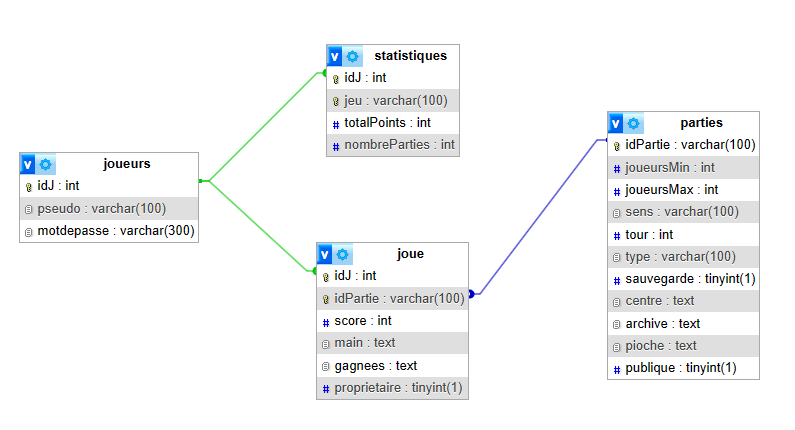
\includegraphics[width=1\textwidth]{bdd.png}
\caption{Schéma de la base de données MySQL.}
\label{fig:bdd}
\end{figure}

Un exemple d'appel à la base de données se situe dans le fichier \texttt{Server/Scripts/GameLogic/utils/functions.js}, des lignes 31 à 46. C'est donc un appel effectué par le serveur NodeJS.\\
\begin{verbatim}
function recupererInfosJoueurs(db, idParty){
    return new Promise((resolve, reject) => {
        db.query('SELECT pseudo,centre,archive,pioche,main,score,tour from parties p,joue j,
            joueurs jo where p.idPartie=j.idPartie and j.idJ=jo.idJ and p.idPartie =?',
            [idParty],async(err,result)=>{
            if(err)reject(err);
            const infosJoueurs=[];
            for(i=0;i<result.length;i++){
                infosJoueurs.push({
                    "nbCards":JSON.parse(result[i].main).length,
                    "pseudo":result[i].pseudo,
                    "score":result[i].score,
                })
            }
            resolve(infosJoueurs);
        });
    });
};
\end{verbatim}
On effectue une requête à la base de données en utilisant la méthode \texttt{db.query(requête, [paramètres], callback)}. Le code a exécuter une fois les données reçues se situe donc dans la fonction de callback.
Dans la fonction recupererInfosJoueurs, utilisée dans plusieurs jeux, on retourne une promesse, qui sera résolue une fois la réponse de la base de données reçue et traitée.
L'utilisation de cette fonction permet de simplifier la récupération des informations des joueurs, comme illustré par l'exemple d'appel ci-dessous :
\begin{verbatim}
    recupererInfosJoueurs(db, "ABCD123").then((infoJoueurs) => {
        // les informations des joueurs sont accessibles dans la variable infoJoueurs
        ...
    }
\end{verbatim}



\subsection{Communication des serveurs} 
\subsubsection{WebSockets}
Plusieurs routes sont utilisées pour communiquer via des WebSockets entre le client et le serveur, en voici une liste non exhaustive.

Du client vers le serveur :
\begin{itemize}
    \item \texttt{playerAction} est envoyé quand un joueur effectue une action. Le client envoie alors le type d'action effectuée, ainsi que les informations spécifiques. Il envoie également son identifiant de joueur ainsi que celui de sa partie.
    \item \texttt{infoGame} est utilisé par le client pour demander au serveur des informations sur la partie dans laquelle il se trouve ; le serveur envoie ensuite les informations par la route \texttt{infoGameOut}.
    \item En Six Qui Prend, lorsqu'un joueur place une carte à faible valeur et qu'il doit ramasser une ligne pour la remplacer par sa carte, la route \texttt{ligne} est utilisée pour informer le serveur du choix effectué par le joueur.
\end{itemize}

Du serveur vers le client :
\begin{itemize}
    \item La route \texttt{newTurn} est utilisée pour envoyer des informations basiques sur le nouveau tour.
    \item Pour des informations plus complètes, c'est la route \texttt{infoGameOut} qui est utilisée.

\begin{verbatim}
const envoyerInfos = async function(db, io, idPartie){
    // On récupère les infos utiles sur la BDD
    db.query('SELECT jo.pseudo as pseudo, jo.idJ as idJ,p.centre,p.archive,j.main,
    j.score,p.type,    FLOOR(COALESCE(s.totalPoints/s.nombreParties, 0))
    as scoreMoyenJoueur,p.pioche FROM parties p JOIN joue j ON p.idPartie = j.idPartie
    JOIN joueurs jo ON j.idJ = jo.idJ LEFT JOIN statistiques s ON j.idJ = s.idJ 
    AND s.jeu = p.type WHERE p.idPartie = ?',[idPartie],async(err,result)=>{
        if(err)reject(err);
        const infoJoueurs=[];
        for(i=0;i<result.length;i++){
            infoJoueurs.push({
                "nbCards":JSON.parse(result[i].main).length,
                "pseudo":result[i].pseudo,
                "score":result[i].score,
                "scoreMoyenJoueur":result[i].scoreMoyenJoueur
            })
        }

        let centre2 = JSON.parse(result[0]["centre"]);
        for(ligne of result){
            centre2[ligne["pseudo"]] = centre2[ligne["idJ"]];
            delete centre2[ligne["idJ"]];
        }
        const draw = JSON.parse(result[0]["pioche"]);
        let nbdraw = draw['pioche']? {'pioche':draw['pioche'].length,
        defausse':draw['defausse'].length}: draw.length;
        // On envoie les informations aux joueurs
        io.to(idPartie).emit('infoGameOut', {center: centre2, 
        archive: JSON.parse(result[0]["archive"]), 
        draw: nbdraw, infoPlayers: infoJoueurs});
    });
}
\end{verbatim}
Dans la fonction envoyerInfos définie dans le fichier \texttt{Server/Scripts/GameLogic/utils/functions.js} des lignes 90 à 114, on récupère les données utiles dans la base de données, avant de les envoyer au client. Dans la ligne \texttt{io.to(idPartie).emit(...)} on constate que la donnée envoyée est un objet ayant des attributs \texttt{center}, \texttt{archive}, \texttt{draw} et \texttt{infoPlayers}.

Après avoir vu la connexion du côté du serveur (NodeJS), penchons-nous sur la connexion du côté du client (React).

Le composant \texttt{SocketProvider} agit comme un fournisseur de connexion, permettant de transmettre l'instance de la socket à l'ensemble de l'application React. Cela garanti que chaque componant puisse utiliser la même connection au serveur et d'éviter d'en recréer une à chaque communication avec le serveur. 

\begin{verbatim}
import io from 'socket.io-client';
const URL = 'http://localhost:3001';
const socket = io(URL);

const SocketProvider = ({ children }) => {
  return (
    <SocketContext.Provider value={{ socket }}>
      {children}
    </SocketContext.Provider>
  );
};

\end{verbatim}

 le composant React appelé `ListParty`  est utilisé pour afficher une liste de parties en attente de joueur ou mise en pause par le joueur et pour cela il se doit de communiquer avec le serveur. Et donc voici un exemple de comment un componant react commmunique avec le serveur :
\begin{verbatim}
function ListParty(props) {
  const {idJ} = usePlayer()
  const [parties, setParties] = useState([]);
  const { socket } = useContext(SocketContext);
  const [error,setError] = useState("")

  useEffect(() => {
    const fetchParties = async () => {
      props.save ?
          socket.on('savedListOut', (data) => {
            setParties(data);
        })
        :socket.on('joinableListOut', (data) => {
            setParties(data);
        });
      props.save ? socket.emit('savedList', idJ) : socket.emit('joinableList');
    };
    
    const cleanup = () => {
      socket.off('joinableListOut');
      socket.off('savedListOut');
    };

    fetchParties();
    return cleanup;
  }, [socket]);
  //rendu
  }
\end{verbatim}

Le composant récupère l'identifiant unique du joueur et la connexion au serveur. Puis, il crée un crochet particulier appelé 'useEffect' qui prend une fonction et une liste de variables. Il surveille le changement de ces variables et se déclenche lorsqu'elles sont modifiées. Ici, lorsque le composant est chargé pour la première fois ou lorsque la connexion change, selon le type de parties spécifiées en paramètre, le useEffect appelle une fonction qui met un écouteur sur une route de sortie et ensuite demande des informations au serveur.

Par exemple, si nous voulons récupérer les parties sauvegardées (c'est-à-dire que l'attribut save est passé à true), nous mettons en place un écouteur sur la route 'savedListOut' et demandons des informations sur 'savedList'. Lorsque des données sont reçues par 'savedListOut', une fonction de callback est déclenchée pour mettre à jour la liste des parties affichées


Une fois le composant démonté, le useEffect va appeler une autre fonction qui va supprimé les écouteur d'évenement, ansi on évite des écoutes multiples et d'écouter lorsque ce n'est plus indispensable.


\end{itemize}
\subsubsection{Requêtes HTTP} Nous n'avons pas utilisé de requêtes HTTP dans le projet, pour garder un fonctionnement homogène dans le traitement de toutes les requêtes.
\subsubsection{Préférences WebSockets/Requêtes HTTP} Nous aurions pu utiliser des requêtes HTTP lors de la soumission de données entrainant un changement de page, par exemple lors de la connexion, ou de la création d'une partie. En revanche, cela n'aurait pas été adapté pour l'envoi de messages dans le chat ou en cas de clic sur une carte.


\section{Utilisation de React}

%Dans cette section, après une  introduction générale d’une ou deux lignes de React, vous %présenterez les aspects saillants de cette technologie en les illustrant par un ou deux composants %React issus de votre projet. Si, en cours de rédaction, vous vous rendez compte que vous n’avez %pleinement tiré parti des facilités offertes par React, vous pouvez signaler à quels endroits de %votre code des 
%modifications auraient été judicieuses
%2 pages maximum hors extrait de code




React.js est un framework JavaScript, développé par Facebook et déployé en 2011, qui permet de créer efficacement des interfaces utilisateur. Il est populaire pour son architecture basée sur des composants, qui se mettent à jour de manière indépendante, optimisant ainsi le rendu des pages HTML.

L'architecture de React permet une modularité intéressante car elle facilite la séparation de la création de composants entre plusieurs personnes. Voici une illustration de ceci :

Nous avons créé des fichiers différents pour chaque jeu avec un composant principal qui décrit son affichage spécifique réalisé par différentes personnes. Par souci de factorisation, tout ce qui était en commun a été extrait et mis dans un composant parent appelé 'GameContainer'. Il réunit toutes les variables globales, le traitement des données envoyées par le serveur et enfin l'affichage de composants nécessaires en tout temps. 'GameContainer' est un composant assez riche et il est difficile à présenter dans son intégralité. L'idée derrière lui est de faciliter l'intégration de nouveaux jeux. Voici une version simplifiée (extrait de \texttt{client/src/Scripts/Shared/gameContainer.js} de la ligne 70 à 231) :

\begin{verbatim}

function GameContainer(){
  const { socket } = useContext(SocketContext);
  const { idParty } = useParams();
  const [cards, setCards] = useState([]);
  const [Info, setInfo] = useState([]);
  const [OtherPlayerAction, setOtherPlayerAction] = useState({});
  const navigate = useNavigate();
  // D'autres états et logiques...
  const contextValue = {
      idParty,
      OtherPlayerAction,
      setOtherPlayerAction,
      Info,
      setInfo,
      cards,
      setCards,   
      socket,
      navigate,
      //reste des états
  }
  useEffect(() => {
    const fetchInfoServ = async () => {
        socket.on('dealingCards', (data) => {
          console.log("Cartes reçues via dealingCards",data);
          setCards(data.Cards);
        });
        //Exemple de mise à jour d'un crochet dans une fonction de callback
        socket.on('conveyAction', (data) => {
            console.log("conveyAction reçu",data);
            setOtherPlayerAction(prevOtherPlayerAction => {
                //création d'une copie pour faire une modification propre
                let copy = {...prevOtherPlayerAction};
                
                //soit on créé un nouvel attribut soit on le met à jour
                copy[data.pseudoJoueur] = data.natureAction;

                //ceci est la nouvelle valeur de otherPlayerAction
                return copy;
            });
        });
        // Autres écouteurs d'événements
        socket.emit('infoGame', idParty);
        socket.emit("requestCards", { "idJ": idJ, "idParty": idParty });//le serveur renvoit sa réponse sur 'dealingCards'
    }
    const cleanup = () => {
        socket.removeAllListeners();
    }
    fetchInfoServ();//fonction exécutée quand le componant est monté
    return cleanup;//fonction a exécuter quand le componant est démonté 
  }, []);//liste des dependences vide afin que cela soit executer seulement à son 1er affichage

    return(
    <>
        <Deconnection />
        <Leave idj={idJ} socket={socket} />
        <Chat data={{ party: idParty }} />
        {resultGame ?
            <EndGame resultGame={resultGame} Info={Info}/>
            :<>
            <Save data={{ party: idParty }}/>
             <Outlet context={contextValue} />//
            </>}
        {Info['nbTour']>=0?<NbTurn nbTurn={Info['nbTour']}/>:<></>}
    </>
    )
}
\end{verbatim}

Chaque composant peut prendre en paramètre un objet qui va correspondre à un ensemble de paramètres appelés propriétés. Dans ce que retourne le composant, nous pouvons en apercevoir un exemple :
\begin{verbatim}
 <Leave idj={idJ} socket={socket} /> //idj={idJ} et socket={socket} sont des propriétés
\end{verbatim}

Pour éviter de devoir transmettre des valeurs communes à différents composants par ces propriétés, 'GameContainer' commence par créer un contexte. Les contextes sont l'équivalent en React des variables globales, tout enfant du contexte peut y accéder. Ils facilitent donc largement la transmission d'information. Pour cela, le composant va récupérer diverses variables des contextes employés avant lui, puis il va instancier des crochets React. Les crochets sont les éléments les plus importants de React car ils sont ce qui fait le dynamisme de React, puisqu'ils sont responsables de l'actualisation des éléments de la page lorsqu'ils sont modifiés. Il va ensuite mettre en place 10 écouteurs d'événements envoyés par le serveur dans un useEffect.\\

Nous avons déjà pu discuter de comment un composant communique avec le serveur dans la partie \textbf{3.3 Communication des serveurs}, mais pour faire un rappel rapide, une première fonction est appelée lors du premier montage du composant mettant en place les écouteurs et une deuxième est appelée lors du démontage pour enlever ces écouteurs une fois obsolètes. Dans la première fonction, il demande au serveur des informations sur les parties avec 'infoGame' (correspond à toutes les informations à afficher) et la liste des cartes que le joueur possède dans sa main. Chaque écouteur va appeler une fonction qui va ensuite mettre à jour un des crochets, relançant un affichage de gameContainer. C'est ici que nous pourrions noter une fragilité de notre code, puisque gameContainer est le composant principal de la page, à chaque changement on relance l'affichage de toute la page sauf que React est sélectif dans son actualisation et les composants qui ne dépendent pas de ce crochets ne sont pas actualisés. Donc le composant est à la fois modulaire et techniquement efficace.\\

Donc, à ce stade, nous avons un composant contenant une connexion au serveur et des écouteurs, ainsi qu'un dictionnaire appelé contextValue contenant lui-même divers crochets et variables. Il affiche un bouton pour se déconnecter, un chat, un bouton pour quitter la partie et le nombre de tours effectués.\\

Mais maintenant, comment afficher un jeu particulier ? Pour cela, nous utilisons la bibliothèque React-Router qui permet, à partir de l'adresse HTTP, de rendre un composant particulier et de récupérer des paramètres dans cette adresse. Nous récupérons ainsi l'identifiant de la partie avec la fonction 'useParams()'. Pour se déplacer entre les différentes routes, nous utilisons 'navigate()'. Ainsi, dans la salle d'attente, une fois la partie lancée, nous envoyons l'utilisateur à l'adresse du jeu. Un exemple serait :

\begin{verbatim}
setTimeout(() => navigate('/Home/Games/Bataille/'+data.idParty), 250);
\end{verbatim}

Ceci déclenche l'affichage du composant parent de la route 'gameContainer' qui, grâce au composant fourni par la bibliothèque :

\begin{verbatim}
 <Outlet context={contextValue} />//
\end{verbatim}

indique où et quand le composant enfant de la route doit s'afficher. De plus, nous passons en propriété la valeur du contexte créé précédemment, permettant à 'Outlet' de créer le contexte utilisable ensuite dans les différents fichiers des jeux.

Nous avons donc pu créer un composant encapsulant la plupart des éléments de logique derrière les jeux facilitant leur ajout tout en maintenant les qualités de React. Il suffit de créer un affichage ou de réutiliser ceux déjà existants et de rendre interactifs les éléments de jeu.

\begin{verbatim}
setTimeout(() => navigate('/Home/Games/Bataille/'+data.idParty), 250);
\end{verbatim}

Ceci déclenche l'affichage du composant parent de la route 'gameContainer' qui, grâce au composant fourni par la bibliothèque :

\begin{verbatim}
 <Outlet context={contextValue} />//
\end{verbatim}

indique où et quand le composant enfant de la route doit s'afficher. De plus, nous passons en propriété la valeur du contexte créé précédemment, permettant à 'Outlet' de créer le contexte utilisable ensuite dans les différents fichiers des jeux.

Nous avons donc pu créer un composant encapsulant la plupart des éléments de logique derriére les jeux facilitant leur ajout tout en maintenant les qualitées de reac. Il suffit de créer un affichage ou de réutiliser ceux déja existant et de rendre interactif les éléments de jeu.





\section{Bilan}

La première semaine, nous n'avons pas été capables de remplir le cahier des charges. En effet, nous n'avons pas réussi à obtenir un affichage fonctionnel de la bataille. Cela a été dû à plusieurs facteurs et a permis une introspection et une amélioration lors de la deuxième semaine. Nous attribuons cet échec à notre manque d'expérience. Il a été difficile de s'organiser, ne connaissant pas le temps nécessaire à chaque tâche, et nous n'avions jamais utilisé GitHub dans le cadre d'un projet de groupe. De plus, nous découvrions aussi React, un framework très riche et très complexe, qui emploie des concepts tout à fait nouveaux. Il nous a donc fallu du temps pour apprendre à coder avec React, utiliser GitHub, mais aussi pour gérer notre temps, à la fois personnel et collectif. Pour la deuxième semaine, nous avons alors formé deux groupes de deux, l'un sur le serveur React, l'autre sur le serveur Node.js. Et nous avons constaté un net progrès puisque cette fois-ci, nous avons fini dans les temps tout en limitant le travail effectué à la maison.

Au fur et à mesure du projet, nous avons réécrit plusieurs fois des extraits de code pour les améliorer et les simplifier. Nous avons ainsi constaté une nette amélioration de la qualité du code entre celui produit lors de la première semaine du projet et celui écrit plus récemment. De plus, nous avons mieux réparti le travail entre les membres du groupe, et ainsi mieux tiré parti des fonctionnalités de l'architecture de gestion de versions proposée par GitHub.

\newpage
\section{Annexe}
\subsection{Ce qui n'a pas été implémenté}
\begin{itemize}
    \item Requêtes HTTP (tout est en websocket)
    \item Délai pour le choix de carte
    \item Client responsive
\end{itemize}
\subsection{Diagrammes de Gantt}

\begin{figure}[ht]
\centering
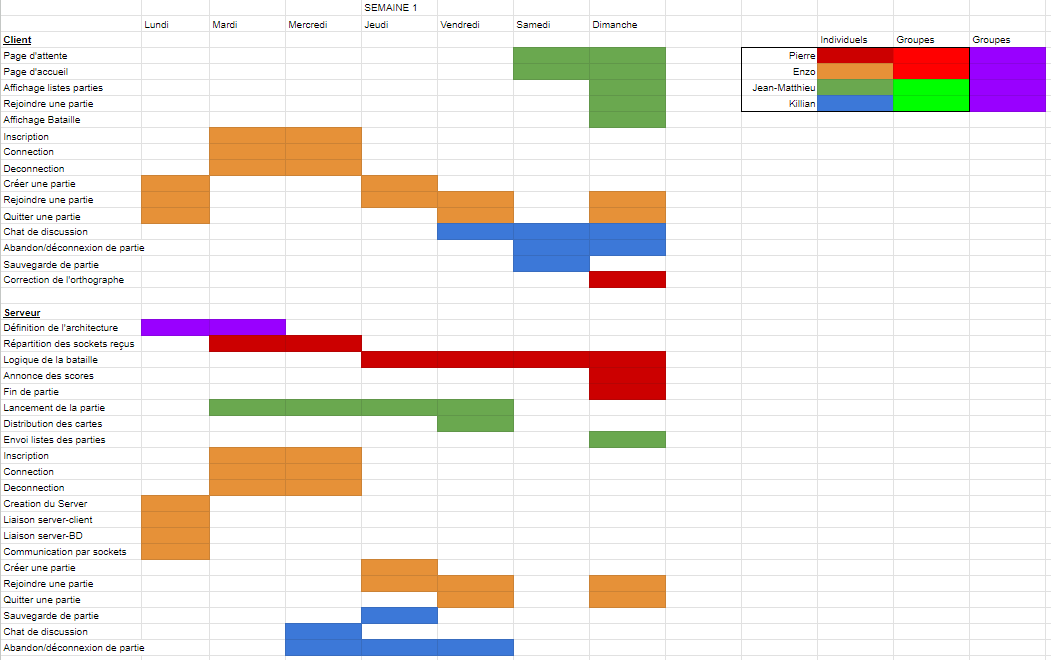
\includegraphics[width=1\textwidth]{semaine1.png}
\caption{Organisation de la première semaine.}
\label{fig:bdd}
\end{figure}

\begin{figure}[ht]
\centering
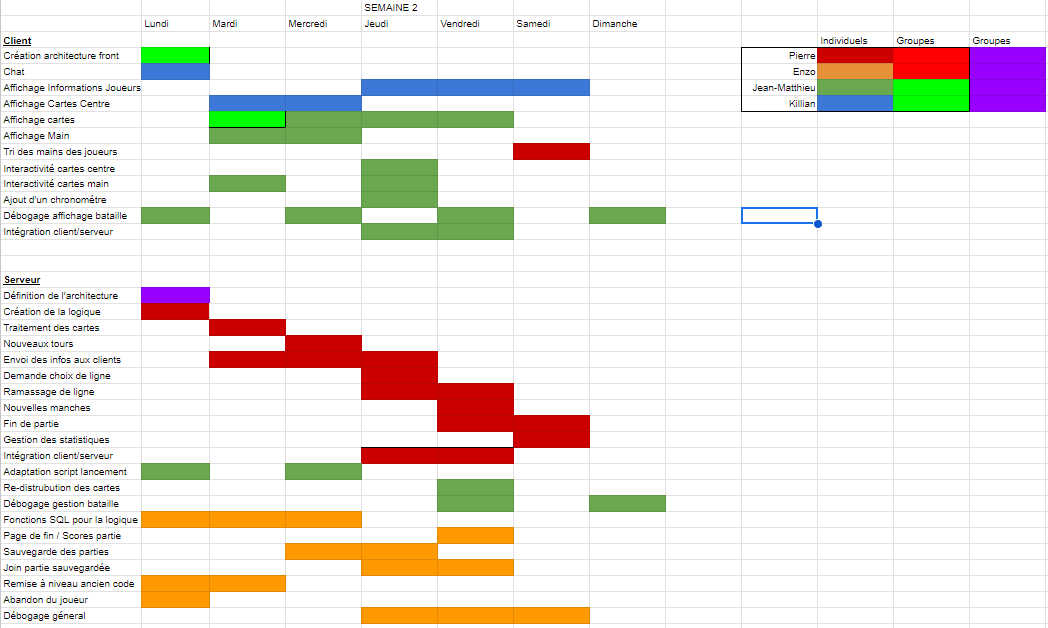
\includegraphics[width=1\textwidth]{semaine2.png}
\caption{Organisation de la deuxième semaine.}
\label{fig:bdd}
\end{figure}
\begin{figure}[ht]
\centering
\includegraphics[width=1\textwidth]{intermede.png}
\caption{Organisation de l'intermède.}
\label{fig:bdd}
\end{figure}
    \end{document}

